% REMEMBER: You must not plagiarise anything in your report. Be extremely careful.
\documentclass{l4proj}

    
%==============================================================================
% Put any additional packages here
% You can add any packages you want, as long as it does not alter
% the overall format (e.g. don't change the margins or the reference style).
%
\usepackage{pdfpages} % if you want to include a PDF for an ethics checklist, for example
%
%

\begin{document}

%==============================================================================
%% METADATA
\title{Programming Language Translation} % change this to your title
\author{Scott Johnston}
\date{September 14, 2018}

\maketitle

%==============================================================================
%% ABSTRACT
\begin{abstract}
With the number of different programming languages available on the market today, all offering different advantages, a programming language translator which would allow code to be converted from one language to another effectively is desirable. For this Honours project, I worked to develop a translation tool using the ANTLR framework, that would allow code in Java to be converted into Python.
Despite their prevalence of these languages in modern programming, the development of this tool is relatively unique. The tool that shall be discussed will allow for code between the two languages to be translated with ease and with decent accuracy, and shows massive potential to be powerful in the future, which will also be discussed in this thesis.


    Every abstract follows a similar pattern. Motivate; set aims; describe work; explain results.
    \vskip 0.5em
    ``XYZ is bad. This project investigated ABC to determine if it was better. 
    ABC used XXX and YYY to implement ZZZ. This is particularly interesting as XXX and YYY have
    never been used together. It was found that  
    ABC was 20\% better than XYZ, though it caused rabies in half of subjects.''
\end{abstract}

%==============================================================================
%% ACKNOWLEDGEMENTS
\chapter*{Acknowledgements}
I would like to thank my supervisor Derek Somerville for his guidance and support over the past year. I really valued the creativity Derek provided, as well as helping me through the unprecedented difficulties provided by the COVID-19 pandemic.

% Enter any acknowledgements here. This is optional; you may leave this blank if you wish,
% or remove the entire chapter
%
% We give thanks to the Gods of LaTeX, who in their eternal graciousness, 
% have granted that this document may compile without errors or overfull hboxes.
%

%==============================================================================

% EDUCATION REUSE CONSENT FORM
% If you consent to your project being shown to future students for educational purposes
% then insert your name and the date below to  sign the education use form that appears in the front of the document. 
% You must explicitly give consent if you wish to do so.
% If you sign, your project may be included in the Hall of Fame if it scores particularly highly.
%
% Please note that you are under no obligation to sign 
% this declaration, but doing so would help future students.
%
\def\consentname {Scott Johnston} % your full name
\def\consentdate {16 February 2021} % the date you agree
%
\educationalconsent


%==============================================================================
\tableofcontents

%==============================================================================
%% Notes on formatting
%==============================================================================
% The first page, abstract and table of contents are numbered using Roman numerals and are not
% included in the page count. 
%
% From now on pages are numbered
% using Arabic numerals. Therefore, immediately after the first call to \chapter we need the call
% \pagenumbering{arabic} and this should be called once only in the document. 
%
%
% The first Chapter should then be on page 1. 

% PAGE LIMITS
% You are allowed 40 pages for a 40 credit project and 30 pages for a 
% 20 credit report. 
% This includes everything numbered in Arabic numerals (excluding front matter) up
% to but *excluding the appendices and bibliography*.
%
% FORMATTING
% You must not alter text size (it is currently 10pt) or alter margins or spacing.
% Do not alter the bibliography style. 
%
%==================================================================================================================================
%
% IMPORTANT
% The chapter headings and structure here are **suggestions**. You don't have to follow this model if
% it doesn't fit your project. Every project should have an introduction and conclusion,
% however.  If in doubt, your supervisor can give you specific guidance; their view takes precedence over
% the structure suggested here.
%
%==================================================================================================================================
\chapter{Introduction}

% reset page numbering. Don't remove this!
\pagenumbering{arabic} 

% You can use \todo{} to mark text that needs to be fixed. Anything inside will appear as highlighted 
% text in the final copy, and you will also get warnings when you compile (so you don't
% forget to take them out!)

\section{Background}
\subsection{Programming Language Translation}
 Program conversion process has been placed  among  the  top  10  challenges  in  the  programming  world  (Terekhov, A. A., & Verhoef, C., (2000) "The realities of language conversions". IEEE  Software,  vol. 17, no. 6, pp. 111-124.) Whilst there exists many tools online to try such a thing, it is an area of research which is yet to be cracked. The motivation for such a tool is clearly there however, due to the amount of research that has been done into conversion tools. There has also been a number of discoveries made into how best to translate code, with a lot of experts agreeing on an intermediate layer between the two languages. This concept is fully explored by Coco, Osman and Osman in their paper "JPT: A Simple Java-Python Translator". This involved the use of an XML middle-layer to try and translate the basic principles of programming languages from Java into Python. As things stand, there are a multitude of translators on the market to and from the most popular programming languages about, however the process of re-engineering certain codes due to the uniqueness of different languages semantics and syntax, has meant that sophisticated code is difficult to convert. 
 
\subsection{Java2Python}
Java2Python is the most recognisable tool that is available, and holds similar abilities to the tool that this project intends to produce. Java2Python uses ANTLR to create an abstract syntax tree from the source code (java file) and walks the tree's nodes, converting each node to it's Python equivalent. This is a similar approach taken in this project, but with some key differences that will be discussed late in the design chapter. Java2Python exists in the Python Package Index (PyPi), meaning it has been recognised by Python themselves, as a useful package. It is described on their website as a tool to "imperfectly translate Java source code to Python source code". This imperfection will also be discussed later in the background chapter of this paper, including the fact it is outdated, it's clear limitations, and it's verbose nature causing confusion.
\subsection{ANTLR and StringTemplate}
The Programming Language translator is built primarily using the ANTLR framework along with stringTemplate.

\subsubsection{ANTLR}

ANTLR stands for "Another Tool for Language Recognition". The framework uses a user-generated grammar file to generate a parser which can then be used for reading, processing, executing, or in this case, translating structured text files. ANTLR was built in Java however has been developed to allow users to use this tool with any type of target language (for example, the Java2Python application built the backend in Python). ANTLR is widely used in academia and industry to build all sorts of tools, frameworks and languages, including the Twitter Search, for query parsing. This shows the power and reach the ANTLR tool has.

\subsubsection{StringTemplate}
StringTemplate is a java template engine which can be used to output source code. A template engine is a code generator that emits text using templates, which are essentially just text documents with spaces for attributes to be added. These attributes will be found via the parser generator (in this case ANTLR) which will direct the attributes to the correct template.
\subsubsection{Combining ANTLR and StringTemplate}
These two softwares collaborated nicely due to stringTemplate powering ANTLR, and justification for how and why they were used can be found in the design and implementation section of this thesis.
To briefly explain it however, there is a Java grammar that exists in ANTLR, which is then parsed, essentially identifying nodes of attributes. These attributes are then fed into the Python StringTemplate to output Python source code. This approach was primarily inspired from the following document, explaining how the two combined to give a very simple translator:
https://theantlrguy.atlassian.net/wiki/spaces/ST/pages/1409118/Language+Translation+Using+ANTLR+and+StringTemplate

\subsection{Impact of COVID-19}
The 2020-21 academic year has been gravely impacted by the ongoing global pandemic. This had an indirect yet significant affect on this honours project. Face-to-face communication has been extremely restricted throughout the year, meaning that meetings with supervisors were limited to online calls via microsoft teams, which many would argue is harder to be engaged with.

On top of this the pandemic situation was anxiety inducing, which many recent studies, including "Onboarding during Covid-19: Create Structure, Connect People and Continue Adapting" by Charles Scott, have proven has lead to students struggling with motivation towards their studies. The university did however regularly update students with advice on coping throughout these troubling times.

Ultimately, this project was not majorly influenced by the global pandemic, as the software tool could be built and evaluated without external tools supplied by the university. In general however, opportunities were restricted, making the likes of interviews very difficult to be carried out.

\section{Problem Space}
\subsection{Java and Python}

The decision to focus on a translator between Java and Python ultimately came from the fact that these are the two most prevalent programming languages in the Computing Science course at University of Glasgow. However there is strong justification for this language choice due to their relevance.

\subsubsection{Python}
Python is a highly popular language for a number of reasons, most notably it is easy to read and write, it is an interpreted language, it is dynamically typed, and it possesses a rich base library and garbage collection feature. (https://python.land/python-tutorial/what-is-python) A paper by Fangohr detailed a comparison carried out between C, MATLAB and Python as teaching languages in engineering. This paper heavily supports that python has an easy-to-use syntax and highlights that python is here to stay in industry, due to it's intuitive nature. A paper titled "An Empirical Comparison of Seven Programming Languages" also mapped the advantages of python performance-wise using empirical data, as it performed amongst the best when put up against 6 other well known programming languages. This evidence of both strong performance and syntactical-ease are enough to justify the importance of Python, thus the decision to use it as the target language for the programming language translator was clear.


\subsubsection{Java}
According to Oracle, 3 billion devices run on Java. This proves it's popularity, probably due to it's many advantageous factors. One major factor being the embrace of object-oriented programming (OOP) in contrast to the procedural programming approach associated with a lot of other languages. Other advantages include Java's platform-independency, it's support for a plethora of libraries being appealing to enterprise computing and Java's support for common programming key issues such as multi-threading and automatic memory management. 

\subsubsection{Translation from Java to Python}
Object-Oriented Programming is at the core of all Java programs, which is untrue for Python, despite having OOP capabilities. Java is restrictive and complex to design in comparison to the intuitive nature of python. Java is also statically typed (meaning that a variable's type must be defined), whilst Python is dynamically typed.

Evidently both Python and Java are powerful and popular for a reason, justifying their place as two of the top languages in the programming world. The differences that have also been highlighted are areas which will make the translation process interesting and justifies that there is enough of a difference between the two languages to make a translation tool worthwhile.

Further justification could come from the legal battle currently ongoing between Oracle (owners of Java) and Google. Oracle want a share of the money Google have made from Android, somewhere in the region of a billion US dollars, because of the several Java APIs that have been re-implemented into Android. This battle has been ongoing for 10 years, with both sides of the debate spending several millions of dollars to fight their case. If Oracle were to win this legal battle, it will likely deter businesses from using Java in the future and they may rush to change the programming language they operate in completely. Python would be one of the obvious alternatives due to it's recent popularity.

\section{Motivation}
Whilst it is not believed that Python will replace Java, given the benefit of some python features highlighted in section 1.2, there is definitely an existing argument as to why people may choose to code in python. Aside from this, Python is also closely related to newly emerging fields in computing science such as the Internet of Things (IoT).

In a 2019 article it was suggested by TIOBE that Python could overtake both Java and C to become the most popular programming language in the world. This was due to the "software engineering boom" which attracted newcomers to programming. To understand a simple program such as "hello world" a java user must understand classes, static methods and packages, whilst a C user is required to understand explicit memory management. A Python user however, simply must understand one single line.
The article goes on to explain how Python is widely regarded the first programming language taught to university students, however not only due to it's simple high-level syntax. It is due to Python being the number one language in a number of different computing domains such as statistical, AI programming, scripting, system tests, web programming and scientific computing.

Figure \ref{fig:index} shows the TIOBE Programming Community index from February 2021. This index is used as indicator of the popularity of programming languages. The ratings use popular search engines to calculate the ratings, and is based on the number of skilled engineers world-wide, courses and third-party vendors. The graphic clearly indicates the rise of Python and relative fall from Java (Despite still being number 2 in the overall rankings). This evidence benefits what was stated in the 2019 article about Python's rise in the next few years.

This evidence combined makes Python a strong candidate to soon dominate the software market. This in turn could create the shift in many different industries from their current software (in a lot of cases a Java software) to one operated in Python. This could become a tedious job, and rewriting software in a new language from scratch would be both time consuming and expensive. Therefore, a mechanism that converts Java (a vastly popular programming language that is starting to wane) to Python (a language which is massively increasing in popularity) relatively accurately and automatically, could be imperative in the software development world in the near future.

\begin{figure}[htb]
    \centering
    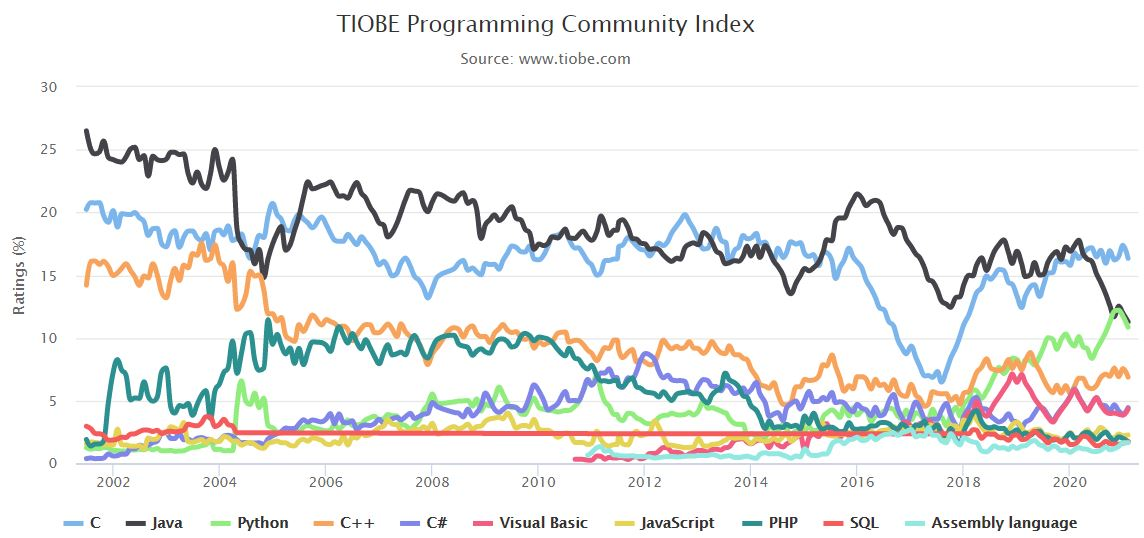
\includegraphics[width=1\linewidth]{images/Programming Community Index.JPG}
        \caption{TIOBE Programming Community Index from February 2021. Focus should be on the green line showing Python's strong growth between 2018-present. 
    }
    \label{fig:index} 
\end{figure}

A paper titles "Python - The Fastest Growing Programming Language" is further evidence for a move to Python. The paper details the many benefits of Python, which have roughly been covered in this paper already. It then goes on to discuss how being able to code in Python is now a more in-demand skill than ever, stating that in terms of search volume, learning Python is the \#1 search when compared to other programming languages. On top of this, Python is an open-source project, with a moderate update cycle, with new versions coming out about once a year. This allows Python to stay relevant which cannot be said about certain other popular languages, with Java updates less regular and significant, and C updates being non-existent.

\section{Research Questions}
As briefly summarised in section 1.3, the overall goal was to try and create a tool which would convert a program written in Java to Python, without compromising accuracy or code quality. Aside from this overall goal, objectives were set out which were altered as the project went on to fit with what had been achieved. 

Upon some background research which shall be touched upon in Section 2,  Program conversion process has been placed  among  the  top  10  challenges  in  the  programming  world (https://ieeexplore.ieee.org/stamp/stamp.jsp?tp=&arnumber=895180), and the comparison of programming language conversion to "turning a sausage into a pig" from the same paper, shows that this was not going to be a straightforward task. A fully functioning translator with 100\% accuracy was not achievable given the time frame and skill level, and some would even argue impossible to ever have such a powerful translator. An example of why this is impossible could be a package with certain capabilities existing in Java but not in Python.

Nevertheless, the following objectives were decided upon:
\begin{itemize}
    \item
    1) Ensure simple/common coding paradigms can be translated (explanation below)
    \item
    2) Ensure the code is expandable for future work.
    \item
    3) Ensure through evaluation that translator is at least as good as what is on the market
    \item
    4) Keep translations as simple as possible 
    \item
    5)
    \item
    6)
\end{itemize}

For the sake of clarity here is a more thorough description of each objective.

For objective \textbf{\#1}, consideration was taken into what is the most useful and common coding patterns used in Java that should be implemented into the translator. Given my own coding experience accompanied by W3Schools.com (which offers tutorials for beginners), these were selected as follows:

Conditional statements in the form of if/else/ else if as well as logical conditions using mathematical symbols (e.g 'a>'b, 'a<b', 'a==b').

Switch statements, which are a form of conditional statement to select a block of code that executes if a case is met (switch/case/default)

While loops, and do/while loops where a block of code will be executed as long as a specified condition is reached.

For loops, where the number of times code will be looped is specified, rather than a condition waiting to be met. Also for-each loops can be used when looping through elements in a list-type structure such as an array.

Also included in this objective, would be converting the OOP structure required in Java into Python, Which meant creating classes and methods in the translation. This is not only good coding practice, but meant the code could be easily compared due to the shape remaining similar.

The ANTLR grammar file used for translation was also imperative in finding what areas of the Java programming language to focus on. This file will be discussed later in the design phase of this thesis.

Objective \textbf{\#2} was actually decided upon during my background research when looking for similar software tools that had been built. Whilst there was some helpful research, a lot of the tools were difficult to use any source code from, due to their unclear structure. 
This meant that even if my translator was just to be a "proof of concept", the way in which it should be built is so that it is extendable, such that the 'future work' set out in this thesis could possibly be built using the framework I have managed to design so far.

For Objective \textbf{\#3}, there was a few translator tools on the market that did a similar thing to what this was intended to do, and decided that for this to be a success, the evaluator should perform at least as well as what is currently on the market. This meant testing my tool with the java2python test folder that can be found at https://github.com/natural/java2python/tree/master/test and I intended for my evaluation to be a success if my tool converted all these tests with accuracy and perhaps could improve upon this tool through a comparison. This objective will be discussed further in the evaluation phase of this thesis.

For Objective \textbf{\#4}, I did not want to make translation overly complicated. A philosophy adopted with this tool from early on was that if the translation can be simplified, it has not been fully successful. This idea came from my evaluation of other translation systems, as I felt some conversions, whilst able to compile and run successfully, the translation looked over complicated and thus, may be too indecipherable and very difficult to maintain and add features to.

\section{Contributions}

\subsection{What has been Learnt}

Programming translation is a topic that on the surface seems relatively straight forward. This project taught the true hardship behind creating a powerful programming language converter, and where issues can occur. It was also an eye opener to some of the great frameworks available and the research into the project which made the future of programming language translation seem somewhat more reachable. It also taugh a lot about how a translator should be evaluated and tested, and at what point the tool can be considered effective.

\subsection{Technologies}
As previously mentioned, ANTLR and StringTemplate were the primary frameworks used for this translator. This is a credit to Terence Parr, a Computer Science professor from the University of San Francisco. His development on language translation tools has been ongoing since 1989, and without his efforts it is likely this project would not have been as successful.
Terence Parr also wrote the article on using ANTLR with StringTemplate, which was very handy in helping with the understanding of connecting the two technologies.
The Java Grammar file used in this project was also taken from the ANTLR github repository and adapted, but without it, the creation of the Java grammar file may have taken a lot longer.

Credit also has to go to Java2Python, as it was helpful in indicating the principles of programming languages that should be focused on. It was also used partially to test the tool that was created, and so without it's test cases, it would have been time consuming to evaluate our translator.

\section{Methodology Summary}
To create this tool I first of all researched the current market of programming language translators. Inspiration from these tools was taken, however they were also criticized for what they lacked, and what could have been improved upon.
This helped lead to the design process, as the criteria was able to be laid down for exactly what was required of the translator.
Once the functional requirements were laid out, research was undertaken to identify what software was available on the market which would offer this functionality. 
Once ANTLR and StringTemplate were identified as reaching these requirements, GitHub was used to find any open source code which could be used for my project.
Once this code was found, and I was familiar with how the software worked, I used this existing code to try and extend it to a translator.
Evaluation was ongoing as I created the tool to ensure the objectives were stuck to closely.

\section{What has been built}
A programming language translator tool has been built, using Java, ANTLR, and StringTemplate frameworks, which is able to translate from Java to Python. The tool is able to translate the majority of Java's in-built functionality to Python in the most minimalist form, so as not to confuse things and means the code is maintainable in the future. The way in which this tool has been built uses a Java Grammar from ANTLR's GitHub repository which I have extended slightly to add some functionality, and a StringTemplate file which was influenced by the StringTemplate GitHub however was primarily built from scratch. This technique of building was chosen due to it's extendability in the future, as this thesis will demonstrate how easily the tool could be expanded in future.

\section{Thesis Outline}
The rest of this paper is structured as follows:
Chapter 2 analyses and critiques the current research in this field, and the current products on the market.
Chapter 3 is a general summary of the method used to decide upon the criteria of the tool and it's evaluation.
Chapter 4 is the analysis and the specification of what is required in a programming language translator.
Chapter 5 details the design process of the translator before being built.
Chapter 6 details the implementation of the translator and any setbacks faced in the building process.
Chapter 7 will detail how the tool was evaluated and how well it performed in the evaluation process.
Chapter 8 will then be the conclusion of the findings from this paper, reflection of the process,  and any future work that could take place in this field.







\todo{Remove the guidance notes from your dissertation before submitting!}

Why should the reader care about what are you doing and what are you actually doing?
\section{Guidance}

\textbf{Motivate} first, then state the general problem clearly. 

\section{Writing guidance}
\subsection{Who is the reader?}

This is the key question for any writing. Your reader:

\begin{itemize}
    \item
    is a trained computer scientist: \emph{don't explain basics}.
    \item
    has limited time: \emph{keep on topic}.
    \item
    has no idea why anyone would want to do this: \emph{motivate clearly}
    \item
    might not know \emph{anything} about your project in particular:
    \emph{explain your project}.
    \item
    but might know precise details and check them: \emph{be precise and
    strive for accuracy.}
    \item
    doesn't know or care about you: \emph{personal discussions are
    irrelevant}.
\end{itemize}

Remember, you will be marked by your supervisor and one or more members
of staff. You might also have your project read by a prize-awarding
committee or possibly a future employer. Bear that in mind.

\subsection{References and style guides}
There are many style guides on good English writing. You don't need to
read these, but they will improve how you write.

\begin{itemize}
    \item
    \emph{How to write a great research paper} \cite{Pey17} (\textbf{recommended}, even though you aren't writing a research paper)
    \item
    \emph{How to Write with Style} \cite{Von80}. Short and easy to read. Available online.
    \item
    \emph{Style: The Basics of Clarity and Grace} \cite{Wil09} A very popular modern English style guide.
    \item
    \emph{Politics and the English Language} \cite{Orw68}  A famous essay on effective, clear writing in English.
    \item
    \emph{The Elements of Style} \cite{StrWhi07} Outdated, and American, but a classic.
    \item
    \emph{The Sense of Style} \cite{Pin15} Excellent, though quite in-depth.
\end{itemize}

\subsubsection{Citation styles}

\begin{itemize}
\item If you are referring to a reference as a noun, then cite it as: ``\citet{Orw68} discusses the role of language in political thought.''
\item If you are referring implicitly to references, use: ``There are many good books on writing \citep{Orw68, Wil09, Pin15}.''
\end{itemize}

There is a complete guide on good citation practice by Peter Coxhead available here: \url{http://www.cs.bham.ac.uk/~pxc/refs/index.html}. 
If you are unsure about how to cite online sources, please see \citet{UNSWWebsite}. 
\footnote{Specifying an online resource like \url{https://developer.android.com/studio}
in a footnote sometimes makes more sense than including it as a formal reference.}

\subsection{Plagiarism warning}

\begin{highlight_title}{WARNING}
    
    If you include material from other sources without full and correct attribution, you are commiting plagiarism. The penalties for plagiarism are severe.
    Quote any included text and cite it correctly. Cite all images, figures, etc. clearly in the caption of the figure.
\end{highlight_title}

\subsection{Quoting text}

If you are quoting a long passage, use a \texttt{quote} environment:

\begin{quote}
     If you scribble your thoughts any which way, your readers will surely feel that you care nothing about them. They will mark you down as an egomaniac or a chowderhead -or, worse, they will stop reading you. The most damning revelation you can make about yourself is that you do not know what is interesting and what is not.
\end{quote} \citep{Von80}

If you are quoting inline, like Simon Peyton-Jones' following remark, use quotation marks ``Conveying the intuition is primary, not
secondary'' \citep{Pey17}.


%==================================================================================================================================
\chapter{Background}
What did other people do, and how is it relevant to what you want to do?
\section{Guidance}
\begin{itemize}    
    \item
      Don't give a laundry list of references.
    \item
      Tie everything you say to your problem.
    \item
      Present an argument.
    \item Think critically; weigh up the contribution of the background and put it in context.    
    \item
      \textbf{Don't write a tutorial}; provide background and cite
      references for further information.
\end{itemize}

%==================================================================================================================================
\chapter{Analysis/Requirements}
What is the problem that you want to solve, and how did you arrive at it?
\section{Guidance}
Make it clear how you derived the constrained form of your problem via a clear and logical process. 

The analysis chapter explains the process by which you arrive at a concrete design. In software 
engineering projects, this will include a statement of the requirement capture process and the
derived requirements.

In research projects, it will involve developing a design drawing on
the work established in the background, and stating how the space of possible projects was
sensibly narrowed down to what you have done.

%==================================================================================================================================
\chapter{Design}
How is this problem to be approached, without reference to specific implementation details? 
\section{Guidance}
Design should cover the abstract design in such a way that someone else might be able to do what you did, 
but with a different language or library or tool. This might include overall system architecture diagrams,
user interface designs (wireframes/personas/etc.), protocol specifications, algorithms, data set design choices,
among others. Specific languages, technical choices, libraries and such like should not usually appear in the design. These are implementation details.


%==================================================================================================================================
\chapter{Implementation}
What did you do to implement this idea, and what technical achievements did you make?
\section{Guidance}
You can't talk about everything. Cover the high level first, then cover important, relevant or impressive details.

\section{General guidance for technical writing}

These points apply to the whole dissertation, not just this chapter.

\subsection{Figures}
\emph{Always} refer to figures included, like Figure \ref{fig:relu}, in the body of the text. Include full, explanatory captions and make sure the figures look good on the page.
You may include multiple figures in one float, as in Figure \ref{fig:synthetic}, using \texttt{subcaption}, which is enabled in the template.


% Figures are important. Use them well.
\begin{figure}[htb]
    \centering
    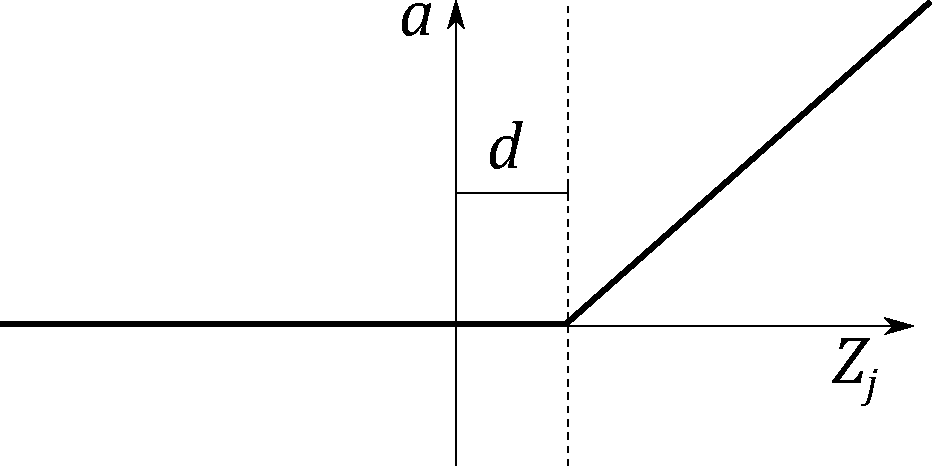
\includegraphics[width=0.5\linewidth]{images/relu.pdf}    

    \caption{In figure captions, explain what the reader is looking at: ``A schematic of the rectifying linear unit, where $a$ is the output amplitude,
    $d$ is a configurable dead-zone, and $Z_j$ is the input signal'', as well as why the reader is looking at this: 
    ``It is notable that there is no activation \emph{at all} below 0, which explains our initial results.'' 
    \textbf{Use vector image formats (.pdf) where possible}. Size figures appropriately, and do not make them over-large or too small to read.
    }

    % use the notation fig:name to cross reference a figure
    \label{fig:relu} 
\end{figure}


\begin{figure}[htb] 
    \centering
    \begin{subfigure}[b]{0.45\textwidth}
        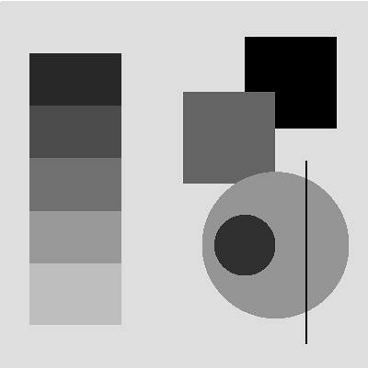
\includegraphics[width=\textwidth]{images/synthetic.png}
        \caption{Synthetic image, black on white.}
        \label{fig:syn1}
    \end{subfigure}
    ~ %add desired spacing between images, e. g. ~, \quad, \qquad, \hfill etc. 
      %(or a blank line to force the subfigure onto a new line)
    \begin{subfigure}[b]{0.45\textwidth}
        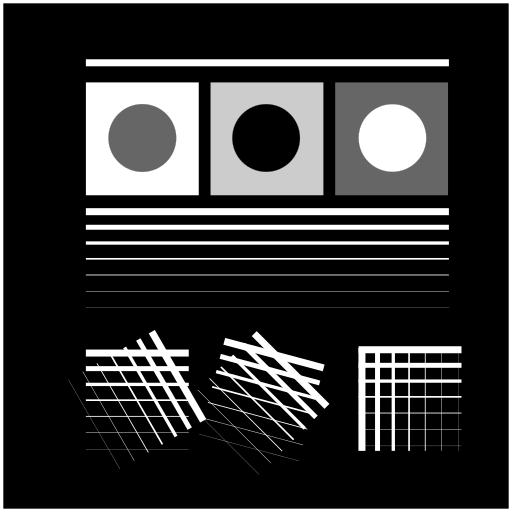
\includegraphics[width=\textwidth]{images/synthetic_2.png}
        \caption{Synthetic image, white on black.}
        \label{fig:syn2}
    \end{subfigure}
    ~ %add desired spacing between images, e. g. ~, \quad, \qquad, \hfill etc. 
    %(or a blank line to force the subfigure onto a new line)    
    \caption{Synthetic test images for edge detection algorithms. \subref{fig:syn1} shows various gray levels that require an adaptive algorithm. \subref{fig:syn2}
    shows more challenging edge detection tests that have crossing lines. Fusing these into full segments typically requires algorithms like the Hough transform.
    This is an example of using subfigures, with \texttt{subref}s in the caption.
    }\label{fig:synthetic}
\end{figure}

\clearpage

\subsection{Equations}

Equations should be typeset correctly and precisely. Make sure you get parenthesis sizing correct, and punctuate equations correctly 
(the comma is important and goes \textit{inside} the equation block). Explain any symbols used clearly if not defined earlier. 

For example, we might define:
\begin{equation}
    \hat{f}(\xi) = \frac{1}{2}\left[ \int_{-\infty}^{\infty} f(x) e^{2\pi i x \xi} \right],
\end{equation}    
where $\hat{f}(\xi)$ is the Fourier transform of the time domain signal $f(x)$.

\subsection{Algorithms}
Algorithms can be set using \texttt{algorithm2e}, as in Algorithm \ref{alg:metropolis}.

% NOTE: line ends are denoted by \; in algorithm2e
\begin{algorithm}
    \DontPrintSemicolon
    \KwData{$f_X(x)$, a probability density function returing the density at $x$.\; $\sigma$ a standard deviation specifying the spread of the proposal distribution.\;
    $x_0$, an initial starting condition.}
    \KwResult{$s=[x_1, x_2, \dots, x_n]$, $n$ samples approximately drawn from a distribution with PDF $f_X(x)$.}
    \Begin{
        $s \longleftarrow []$\;
        $p \longleftarrow f_X(x)$\;
        $i \longleftarrow 0$\;
        \While{$i < n$}
        {
            $x^\prime \longleftarrow \mathcal{N}(x, \sigma^2)$\;
            $p^\prime \longleftarrow f_X(x^\prime)$\;
            $a \longleftarrow \frac{p^\prime}{p}$\;
            $r \longleftarrow U(0,1)$\;
            \If{$r<a$}
            {
                $x \longleftarrow x^\prime$\;
                $p \longleftarrow f_X(x)$\;
                $i \longleftarrow i+1$\;
                append $x$ to $s$\;
            }
        }
    }
    
\caption{The Metropolis-Hastings MCMC algorithm for drawing samples from arbitrary probability distributions, 
specialised for normal proposal distributions $q(x^\prime|x) = \mathcal{N}(x, \sigma^2)$. The symmetry of the normal distribution means the acceptance rule takes the simplified form.}\label{alg:metropolis}
\end{algorithm}

\subsection{Tables}

If you need to include tables, like Table \ref{tab:operators}, use a tool like https://www.tablesgenerator.com/ to generate the table as it is
extremely tedious otherwise. 

\begin{table}[]
    \caption{The standard table of operators in Python, along with their functional equivalents from the \texttt{operator} package. Note that table
    captions go above the table, not below. Do not add additional rules/lines to tables. }\label{tab:operators}
    %\tt 
    \rowcolors{2}{}{gray!3}
    \begin{tabular}{@{}lll@{}}
    %\toprule
    \textbf{Operation}    & \textbf{Syntax}                & \textbf{Function}                            \\ %\midrule % optional rule for header
    Addition              & \texttt{a + b}                          & \texttt{add(a, b)}                                    \\
    Concatenation         & \texttt{seq1 + seq2}                    & \texttt{concat(seq1, seq2)}                           \\
    Containment Test      & \texttt{obj in seq}                     & \texttt{contains(seq, obj)}                           \\
    Division              & \texttt{a / b}                          & \texttt{div(a, b) }  \\
    Division              & \texttt{a / b}                          & \texttt{truediv(a, b) } \\
    Division              & \texttt{a // b}                         & \texttt{floordiv(a, b)}                               \\
    Bitwise And           & \texttt{a \& b}                         & \texttt{and\_(a, b)}                                  \\
    Bitwise Exclusive Or  & \texttt{a \textasciicircum b}           & \texttt{xor(a, b)}                                    \\
    Bitwise Inversion     & \texttt{$\sim$a}                        & \texttt{invert(a)}                                    \\
    Bitwise Or            & \texttt{a | b}                          & \texttt{or\_(a, b)}                                   \\
    Exponentiation        & \texttt{a ** b}                         & \texttt{pow(a, b)}                                    \\
    Identity              & \texttt{a is b}                         & \texttt{is\_(a, b)}                                   \\
    Identity              & \texttt{a is not b}                     & \texttt{is\_not(a, b)}                                \\
    Indexed Assignment    & \texttt{obj{[}k{]} = v}                 & \texttt{setitem(obj, k, v)}                           \\
    Indexed Deletion      & \texttt{del obj{[}k{]}}                 & \texttt{delitem(obj, k)}                              \\
    Indexing              & \texttt{obj{[}k{]}}                     & \texttt{getitem(obj, k)}                              \\
    Left Shift            & \texttt{a \textless{}\textless b}       & \texttt{lshift(a, b)}                                 \\
    Modulo                & \texttt{a \% b}                         & \texttt{mod(a, b)}                                    \\
    Multiplication        & \texttt{a * b}                          & \texttt{mul(a, b)}                                    \\
    Negation (Arithmetic) & \texttt{- a}                            & \texttt{neg(a)}                                       \\
    Negation (Logical)    & \texttt{not a}                          & \texttt{not\_(a)}                                     \\
    Positive              & \texttt{+ a}                            & \texttt{pos(a)}                                       \\
    Right Shift           & \texttt{a \textgreater{}\textgreater b} & \texttt{rshift(a, b)}                                 \\
    Sequence Repetition   & \texttt{seq * i}                        & \texttt{repeat(seq, i)}                               \\
    Slice Assignment      & \texttt{seq{[}i:j{]} = values}          & \texttt{setitem(seq, slice(i, j), values)}            \\
    Slice Deletion        & \texttt{del seq{[}i:j{]}}               & \texttt{delitem(seq, slice(i, j))}                    \\
    Slicing               & \texttt{seq{[}i:j{]}}                   & \texttt{getitem(seq, slice(i, j))}                    \\
    String Formatting     & \texttt{s \% obj}                       & \texttt{mod(s, obj)}                                  \\
    Subtraction           & \texttt{a - b}                          & \texttt{sub(a, b)}                                    \\
    Truth Test            & \texttt{obj}                            & \texttt{truth(obj)}                                   \\
    Ordering              & \texttt{a \textless b}                  & \texttt{lt(a, b)}                                     \\
    Ordering              & \texttt{a \textless{}= b}               & \texttt{le(a, b)}                                     \\
    % \bottomrule
    \end{tabular}
    \end{table}
\subsection{Code}

Avoid putting large blocks of code in the report (more than a page in one block, for example). Use syntax highlighting if possible, as in Listing \ref{lst:callahan}.

\begin{lstlisting}[language=python, float, caption={The algorithm for packing the $3\times 3$ outer-totalistic binary CA successor rule into a 
    $16\times 16\times 16\times 16$ 4 bit lookup table, running an equivalent, notionally 16-state $2\times 2$ CA.}, label=lst:callahan]
    def create_callahan_table(rule="b3s23"):
        """Generate the lookup table for the cells."""        
        s_table = np.zeros((16, 16, 16, 16), dtype=np.uint8)
        birth, survive = parse_rule(rule)

        # generate all 16 bit strings
        for iv in range(65536):
            bv = [(iv >> z) & 1 for z in range(16)]
            a, b, c, d, e, f, g, h, i, j, k, l, m, n, o, p = bv

            # compute next state of the inner 2x2
            nw = apply_rule(f, a, b, c, e, g, i, j, k)
            ne = apply_rule(g, b, c, d, f, h, j, k, l)
            sw = apply_rule(j, e, f, g, i, k, m, n, o)
            se = apply_rule(k, f, g, h, j, l, n, o, p)

            # compute the index of this 4x4
            nw_code = a | (b << 1) | (e << 2) | (f << 3)
            ne_code = c | (d << 1) | (g << 2) | (h << 3)
            sw_code = i | (j << 1) | (m << 2) | (n << 3)
            se_code = k | (l << 1) | (o << 2) | (p << 3)

            # compute the state for the 2x2
            next_code = nw | (ne << 1) | (sw << 2) | (se << 3)

            # get the 4x4 index, and write into the table
            s_table[nw_code, ne_code, sw_code, se_code] = next_code

        return s_table

\end{lstlisting}

%==================================================================================================================================
\chapter{Evaluation} 
How good is your solution? How well did you solve the general problem, and what evidence do you have to support that?

\section{Guidance}
\begin{itemize}
    \item
        Ask specific questions that address the general problem.
    \item
        Answer them with precise evidence (graphs, numbers, statistical
        analysis, qualitative analysis).
    \item
        Be fair and be scientific.
    \item
        The key thing is to show that you know how to evaluate your work, not
        that your work is the most amazing product ever.
\end{itemize}

\section{Evidence}
Make sure you present your evidence well. Use appropriate visualisations, 
reporting techniques and statistical analysis, as appropriate. The point is not
to dump all the data you have but to present an argument well supported by evidence gathered.

If you use numerical evidence, specify reasonable numbers of significant digits; don't state ``18.41141\% of users were successful'' if you only had 20 users. If you average \textit{anything}, present both a measure of central tendency (e.g. mean, median) \textit{and} a measure of spread (e.g. standard deviation, min/max, interquartile range).

You can use \texttt{siunitx} to define units, space numbers neatly, and set the precision for the whole LaTeX document. 

% setup siunitx to have two decimal places
\sisetup{
	round-mode = places,
	round-precision = 2
}

For example, these numbers will appear with two decimal places: \num{3.141592}, \num{2.71828}, and this one will appear with reasonable spacing \num{1000000}.



If you use statistical procedures, make sure you understand the process you are using,
and that you check the required assumptions hold in your case. 

If you visualise, follow the basic rules, as illustrated in Figure \ref{fig:boxplot}:
\begin{itemize}
\item Label everything correctly (axis, title, units).
\item Caption thoroughly.
\item Reference in text.
\item \textbf{Include appropriate display of uncertainty (e.g. error bars, Box plot)}
\item Minimize clutter.
\end{itemize}

See the file \texttt{guide\_to\_visualising.pdf} for further information and guidance.

\begin{figure}[htb]
    \centering
    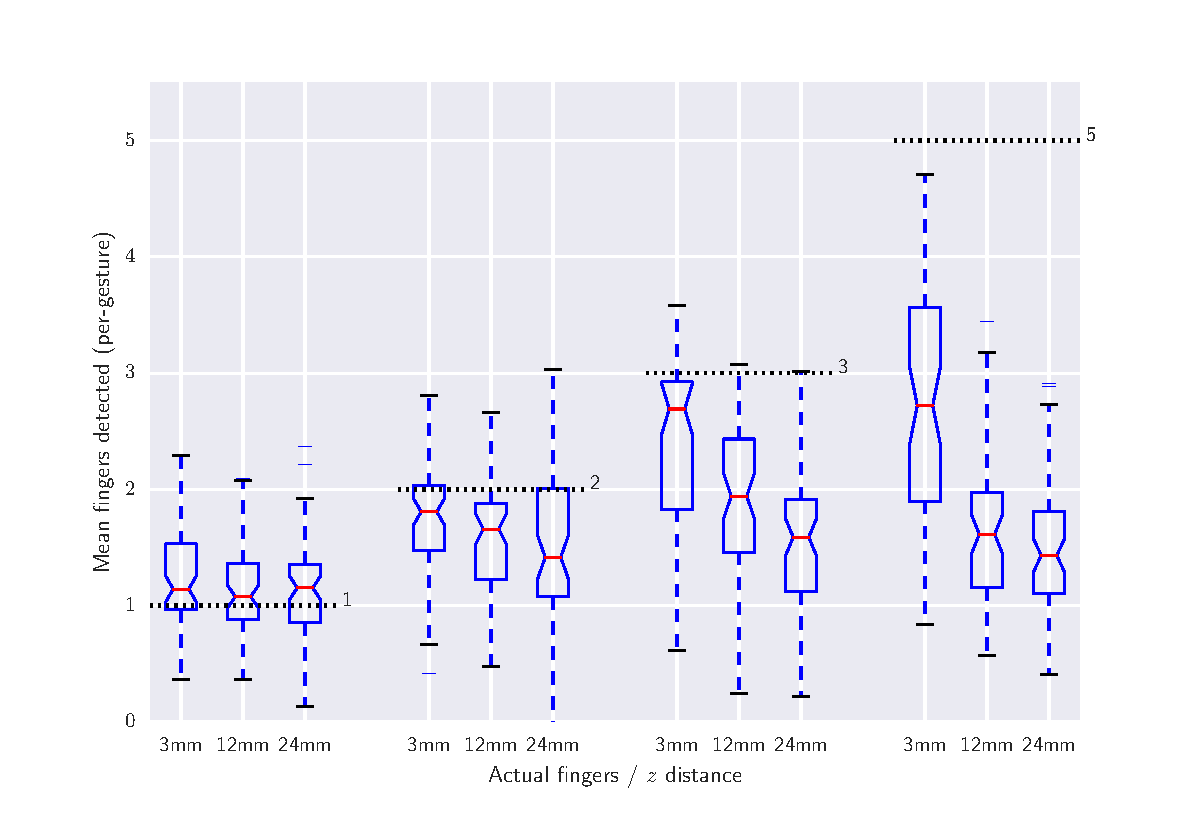
\includegraphics[width=1.0\linewidth]{images/boxplot_finger_distance.pdf}    

    \caption{Average number of fingers detected by the touch sensor at different heights above the surface, averaged over all gestures. Dashed lines indicate
    the true number of fingers present. The Box plots include bootstrapped uncertainty notches for the median. It is clear that the device is biased toward 
    undercounting fingers, particularly at higher $z$ distances.
    }

    % use the notation fig:name to cross reference a figure
    \label{fig:boxplot} 
\end{figure}


%==================================================================================================================================
\chapter{Conclusion}    
Summarise the whole project for a lazy reader who didn't read the rest (e.g. a prize-awarding committee). This chapter should be short in most dissertations; maybe one to three pages.
\section{Guidance}
\begin{itemize}
    \item
        Summarise briefly and fairly.
    \item
        You should be addressing the general problem you introduced in the
        Introduction.        
    \item
        Include summary of concrete results (``the new compiler ran 2x
        faster'')
    \item
        Indicate what future work could be done, but remember: \textbf{you
        won't get credit for things you haven't done}.
\end{itemize}

\section{Summary}
Summarise what you did; answer the general questions you asked in the introduction. What did you achieve? Briefly describe what was built and summarise the evaluation results.

\section{Reflection}
Discuss what went well and what didn't and how you would do things differently if you did this project again.

\section{Future work}
Discuss what you would do if you could take this further -- where would the interesting directions to go next be? (e.g. you got another year to work on it, or you started a company to work on this, or you pursued a PhD on this topic)

%==================================================================================================================================
%
% 
%==================================================================================================================================
%  APPENDICES  

\begin{appendices}

\chapter{Appendices}

Use separate appendix chapters for groups of ancillary material that support your dissertation. 
Typical inclusions in the appendices are:

\begin{itemize}
\item
  Copies of ethics approvals (you must include these if you needed to get them)
\item
  Copies of questionnaires etc. used to gather data from subjects. Don't include
  voluminous data logs; instead submit these electronically alongside your source code.
\item
  Extensive tables or figures that are too bulky to fit in the main body of
  the report, particularly ones that are repetitive and summarised in the body.
\item Outline of the source code (e.g. directory structure), 
    or other architecture documentation like class diagrams.
\item User manuals, and any guides to starting/running the software. 
Your equivalent of \texttt{readme.md} should be included.

\end{itemize}

\textbf{Don't include your source code in the appendices}. It will be
submitted separately.



\end{appendices}

%==================================================================================================================================
%   BIBLIOGRAPHY   

% The bibliography style is agsm (Harvard)
% The bibliography always appears last, after the appendices.

\bibliographystyle{agsm}

% Force the bibliography not to be numbered
\renewcommand{\thechapter}{0} 
\bibliography{l4proj}

\end{document}
